\documentclass[../zhang_thesis.tex]{subfiles}
\begin{document}

\chapter{Introduction}

Batteries, particularly rechargeable ones, are used extensively in daily life. They provide the energy for such electrical systems as communication, automotive, and renewable power systems, among others. In order to design for and operate these systems, an accurate battery model and a means of simulating the model efficiently is needed. For example, modern battery charge and health management schemes use high-fidelity battery models to track the state of charge (SOC) and state of
health (SOH); this information is then used to predict and optimize runtime of the battery. However, most batteries have nonlinear capacitive effects, which require the use of a nonlinear filter. This thesis provides one possible solution to this problem by choosing an appropriate battery model and testing the speed and accuracy of various nonlinear filters in determining the SOC.

%%%%%%%%%%%%%%%%%%%%%%%%%%%%%%%%%%%%%%%%%%%%%%%%%%%%%%%%%%%%%%%

\section{Electrical Characteristics of Rechargeable Batteries}

A high-fidelity battery model has to accurately reproduce the various characteristics of the battery. The characteristics included in most models are the capacity and the state of charge. More accurate models include nonlinear effects, such as the rate-capacity effect and the recovery effect, along with self-discharge and the effects of ambient temperature. The dynamic electrical attributes, such as the current-voltage (i-v) characteristics and transient responses, can also be modeled.

The capacity of a battery is the amount of electric charge it can store, measured in the SI unit Ampere-hours (Ah). Commonly, for rechargeable battery specifications, the subunit milliampere-hour (mAh) is used. Due to the electrochemical nature of batteries, a battery's available capacity decreases as the rate of discharge increases. Therefore, the capacity for a battery is typically stated for a given discharge rate. For lead-acid batteries, this diminishing capacity with increasing discharge rate is known as Peukert's law, which states that for a one-ampere discharge rate~\cite{doerffel06}
\begin{equation}
C_p = I^k t,
\end{equation}
where $C_p$ is the capacity at a one-ampere discharge rate in Ah, $I$ is the discharge current in A, $t$ is the time to discharge the battery in hours, and $k>=1$ is the dimensionless Peukert constant, typically between 1.1 and 1.3 for a lead-acid battery. The constant $k$ only equals unity for an ideal accumulator, so for real batteries, $k$ is always greater than unity. Thus, for a given increase in the discharge current, the discharge time decreases by a proportionally greater amount. Therefore, the effective, or available, capacity $Ct$ is reduced. For a general battery, this effect is known as the rate-capacity effect. Related to this is the recovery effect, so called because when a battery is allowed to rest during an idle period, the battery ``recovers'' available capacity previously lost during discharge due to the rate-capacity effect.

Both the rate-capacity effect and the recovery effect can be explained by the electrochemical nature of the battery. During discharge the concentration of the active material around the electrode is depleted and the active materials in the depletion region move towards the electrode to reduce the concentration gradient~\cite{chiasserini99}. Because the speed at which the concentration gradient is equalized is limited, the faster the rate of discharge, the less active material has been replenished, resulting in a decrease in the capacity. Likewise, when the battery is allowed to rest, the active material gradient has additional time to equalize and increase the available capacity.

Closely related to the capacity is the SOC. This thesis defines it as the ratio between the remaining capacity and the maximum capacity, with both capacities measured using the amount of active material within the battery. This definition then denotes the proportion of remaining chemical energy rather the available energy and is unaffected by the rate-capacity and recovery effects. Note that a fully charged battery has an SOC of unity and a fully discharged battery has an SOC of
zero, regardless of the available capacity. Additionally, it is convenient to establish the relationship between the SOC of the battery and its open-circuit voltage $V_{OC}$, which is useful for simulation of the i-v characteristics and transient responses. $V_\text{OC}$ can be thought as the limit of the measured battery voltage after recovery.

Other more minor effects that are usually incorporated into models are self-discharge, the effect of ambient temperature, and aging. Self-discharge refers to an idle battery decreasing its SOC over time due to internal chemical reactions. It is dependent on the type of battery, SOC, ambient temperatures, and other factors. The ambient temperature has effects on the internal resistance of the battery and the self-discharge rate. Commonly, the battery is designed to operate with a narrow range of temperatures. Below the operating temperature range, the internal resistance increases, decreasing the capacity. Above the operating range, the internal resistance decreases, not only increasing the capacity but also the self-discharge rate; thus, the actual capacity is lowered due to the increased self-discharge. Aging refers to the decrease in battery performance measures, such as capacity, self-discharge, and internal resistance, over time due to unwanted chemical reactions. In practice, aging is indicated by the SOH, defined as the ratio between the current maximum capacity and that of a new battery. The SOH threshold at which the battery performance is considered too degraded varies by application.

\emph{[Where does this go?]} This thesis studied the prediction of the SOC of a battery using noisy measurements of its current and voltage. To do so accurately for a general load, incorporation of the rate-capacity and recovery effects as well as the transient i-v characteristics is desirable. Furthermore, it is useful to have a model easily tunable for different battery types. The following section reviews the characteristics of different battery models and chooses the one most suitable for the purposes of this
study.

%%%%%%%%%%%%%%%%%%%%%%%%%%%%%%%%%%%%%%%%%%%%%%%%%%%%%%%%%%%%%%%

\section{Battery Models}

Battery models can be divided into five categories, namely electrochemical, computational intelligence, analytical, stochastic, and electrical-circuit. The remainder of this section reviews each type and determines the most suitable battery model for this study..

\subsection{Electrochemical}

Electrochemical models are describe the chemical processes that place in the battery in great detail. These are generally the most accurate, but they require in-depth knowledge of the chemical processes to create and impose large computational costs~\cite{jongerden09}. One of the most widely known electrochemical models was developed by Doyle, Fuller, and Newman for lithium and lithium-ion batteries using noninvasive voltage-current cycling
experiments~\cite{doyle93,fuller94,fuller94b}. It consists of six coupled, nonlinear differential equatons that capture lithium diffusion dynamics and charge transfer kinetics. The model is able to predict i-v response and provides a design guide for thermodynamics, kinetics, and transport across electrodes. A implementation of their model in Fortran, called Dualfoil, is available for free online.\footfullcite{newman98} The program needs more than 60 parameters along with the load profile
in order to compute the battery properties. Setting the parameters requires detailed knowledge of the battery, but the result of the program is highly accurate. Other battery models are often compared to it rather than to experimental results.

\subsection{Computational Intelligence}

Computational intelligence is a brance of computer science interested in problems that require the intelligence of humans and animals to solve. One of the earliest definitions by Bezdek states that computational intelligent systems use pattern recognition on low-level, numerical data and do not use knowledge as with artificial intelligence~\cite{bezdek92,bezdek94}. Methods such as neural networks, fuzzy systems, and evolutionary computation are commonly classified as computational
intelligence. Battery models using such methods as neural networks~\cite{ogorman98,capizzi11}, support vector machines~\cite{wang06}, and hybrid neural-fuzzy models~\cite{shen02} have been studied. These models learn the nonlinear relationships between battery properties, such as SOC, current, voltage, and temperature, through a computationally costly training process. However, once trained, they incur a much lower cost and can achieve comparable accuracy to electrochemical
models.

\subsection{Analytical}

\emph{[Needs rewrite to include more detail, eg equations]}

\subsubsection{Peukert's Law}

Analytical models are simplified electrochemical models that trade off accuracy for simplicity. One of the simplest such models is Peukert's law, described above. It is able to model the rate-capacity effect but not the recovery effect. More complicated models, such as the kinetic battery model and the diffusion model, are able to describe both the rate-capacity effect and the recovery effect. However, the current examples of analytical models cannot describe the transient i-v characteristics of batteries.

\subsubsection{Kinetic Battery Model}

The kinetic battery model (KiBaM), initially created for large lead-acid batteries, describes the battery as a kinetic process, using two charge wells for the bound and available charges connected by a valve whose flow rate is proportional to the height difference between the wells~\cite{manwell93}. 

\emph{[Equation that is referenced in the next section.]}
The change of charge in the wells is given by
\begin{equation}
    \begin{cases}
        \frac{dy_1}{dt} = -I + k \left( h_2 - h_1 \right) \\
        \frac{dy_2}{dt} = -k \left( h_2 - h_1 \right),
    \end{cases}
    \label{eq:kibam}
\end{equation}
where $y_1,y_2$ are the charges, $h_1,h_2$ are the heights of the wells, the parameter $k$ controls the rate of charge flow between the wells, and $I$ is the applied load.

The flow rate of the valve should be lower than the typical discharge rate of the battery. During discharge from the available-charge well, the bound charges flow through the valve to equalize the heights of the two wells. It can be seen that for slower discharge
rates, more charge flows through the valve and the effective capacity increases. Likewise, during idle periods for the battery, the available charge increases. Thus, the model is able to describe the rate-capacity and recovery effects.

\subsubsection{Diffusion Model}

Related to the kinetic battery model is the diffusion model, which describes the movement of the ions in the electrolyte of a lithium-ion battery~\cite{rakhmatov01}. Like in the kinetic battery model, the difference in the concentration of adjacent ions along the length of the battery determines the diffusion rate of the ions. The available charges are those ions directly touching the electrode of the battery. It can be seen that the kinetic battery model is a first-order approximation of the diffusion
model~\cite{jongerden09}, so naturally the diffusion model also describes the rate-capacity and recovery effects.

\subsection{Stochastic}

Stochastic models describe the discharging and the recovery effect as stochastic processes. The first models were developed by Chiasserini and Rao and based on discrete-time Markov chains~\cite{chiasserini99b}. They studied two models of a battery in a communication device that transmitted packets. The simpler model described the battery as a discrete-time Markov chain with $N+1$ states, numbered from $0$ to $N$ and corresponding to the number of charge units available in the battery.
Transmitting one packet requires one charge unit of energy. Thus, in continuous transmission, $N$ packets can be sent. At every time step, a charge unit is either consumed with probability $a_1=q$ or recovered with probability $a_0=1-q$. The battery is considered empty when the $0$ state is reached or when a theoretical maximum of $T$ charge units have been consumed. The second model is an extension of the first, allowing for more than one charge unit to be consumed in a time step, modeling
more bursty usage. Additionally, the battery has a non-zero probability of staying in the same charge state, indicating no consumption or recovery during a time step. Chiasserini and Rao extended their model further in following papers by adding state and phase dependence~\cite{chiasserini99,chiasserini01,chiasserini01b}. The state number is the number of charge units, and the phase number is the number of consumed charge units. Having fewer charge units decreases the probability of
recovery, while having more consumed charge units increases the probability of recover. Using these models, one can model different loads by setting the transitions probabilities. However, the order of the transitions is uncontrollable, so it is impossible to model fixed load patterns and compute their impact on battery life.

Chiasserini and Rao mainly investigated the gain $G$ in transmitted packets using a pulsed discharge relative to using a constant discharge, defined as $G=m/N$, where $m$ is the mean number of transmitted packets. The gain increases when the load decreases, due to an increase in the recovery probability. Additionally, the gain increases for lower discharge demand rates and higher current densities. These load profiles result in discharge currents close to the specified limits of the battery, causing the
available capacity to decrease overly quickly. Therefore, the recovery effect is especially strong for these cases during pulsed discharge, greatly increasing the gain. Chiasserini and Rao compared the computation of the gain parameter for different current densities and demand rates using the stochastic model to that of the electrochemical model of Doyle et al. They found an average deviation of 1\% and a maximum deviation of 4\%. This shows that the stochastic model accurately describes battery behavior during pulsed discharge. However, this model is only able to compute relative lifetimes.

In 2005, Rao et al.~\cite{rao05} proposed a stochastic battery model based on the Kinetic Battery Model (KiBaM) of Manwell and McGowan. This stochastic KiBaM was for a nickel-metal hydride (NiMH) battery. The differential equations governing the original KiBaM were modified to include an extra factor $h_2$ governing the flow of charge between the wells. This changes \autoref{eq:kibam} into
\begin{equation}
    \begin{cases}
        \frac{dy_1}{dt} = -I + k_s h_2 \left( h_2 - h_1 \right) \\
        \frac{dy_2}{dt} = -k_s h_2 \left( h_2 - h_1 \right),
    \end{cases}
\end{equation}
This change causes the recovery effect to weaken as the remaining charge decreases. The stochastic model was also modified to allow the possibility of no recovery during idle periods. The stochastic KiBaM describes the battery using a discrete-time, transient Markov process. The states are labeled with the parameters $(i,j,t)$, with $i$ and $j$ representing the discrete charge levels of the available and bound charge wells and $t$ representing the length of the current idle period.
Like the stochastic model of Chiasserini and Rao, it is impossible to fully model a real-life discharge pattern using the stochastic KiBaM. Rao et al.\ compared the results of their model with experimental results using an AAA NiMH battery. Two sets of experiments were conducted, the first with varying frequency of the load and a 50\% duty cycle and the second with varying off-time and a constant on-time. Their model accurately predicted the lifetime and delivered charge from the
battery, with a maximum error of 2.65\%.

\subsection{Electrical-Circuit}

One of the earliest investigations into using electrical circuits to represent batteries came about from a desire to represent impedance spectra created using electrochemical impedance spectroscopy (EIS). There are several major chemical processes within a battery with different time constants. Short-term processes include electric and magnetic, electric double layer, and mass transport effects; long-term processes include cyclical effects based on SOC, reversible effects such
as acid stratification and memory effects, and the irreversible aging effect~\cite{jossen06}. It is convenient to visualize the resultant complex spectra using a Nyquist plot, such as the one shown in \autoref{fig:nyquist_plot_batt}.As shown, the impedance can be divided into three parts, based on the frequency. The approximately linear low frequency portion, on the order of $10^{-6}$ to $10^0$ Hz, is caused by mass transport effects like diffusion. The middle frequency
range, on the order of $10^0$ to $10^3$ Hz and in the shape of a semicircle, is caused by charge transfer and the electrochemical double layer effects. The remaining high frequency portion, on the order of $10^3$ to $10^4$ Hz, is a combination of the conductance and the skin effect.

In 1947, Randles proposed an equivalent electrical circuit to model interfacial electrochemical reactions~\cite{randles47}. His circuit, shown in \autoref{fig:randles_circuit}, consists of the electrolyte resistance $R_s$ in series with the parallel combination of the double-layer capacitance $C_{dl}$ and the impedance of the charge transfer resistance $R_{ct}$ and the Warburg diffusion element $Z_W$. It is one of the simplest methods to interpret the results of
EIS. Recently, Randles' circuit was used to study lithium-ion batteries.

\begin{figure}[htb]
    \centering
    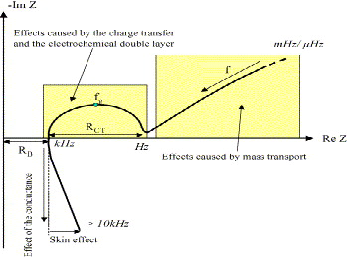
\includegraphics[width=0.8\textwidth]{nyquist_plot_batt}
    \caption{Illustrative Nyquist plot of a battery~\cite{jossen06}. \emph{[Quite low quality from screen capture of article preview. I can recapture for better quality or recreate it.]}}
    \label{fig:nyquist_plot_batt}
\end{figure}

\begin{figure}[htb]
    \centering
    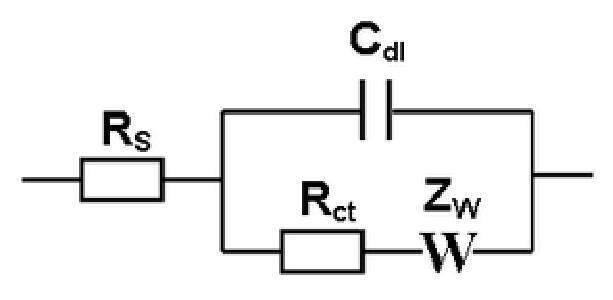
\includegraphics[width=0.6\textwidth]{randles_circuit}
    \caption{Randles' equivalent circuit.}
    \label{fig:randles_circuit}
\end{figure}

In 1993, Hageman created simplified electrical-circuit models using PSpice for nickel-cadmium (NiCd), lead-acid, and alkaline batteries~\cite{hageman93}. The circuits shared the common elements of
\begin{enumerate*}[label=\emph{\roman*})]
\item a capacitor that represents the battery capacity,
\item a discharge rate normalizer that determines the additional capacity loss at high discharge rates,
\item a circuit that discharges the battery,
\item a lookup table of battery voltage versus SOC, and
\item a resistor that represents the battery's internal resistance~\cite{hageman93,hageman97}.
\end{enumerate*}
In addition, battery models for NiCd batteries simulated the thermal effects under high discharge rates. The main lookup table is formed by discharging a battery at a low rate at a constant current (20 to 200 hours). At high discharge rates, the discharge rate normalizer reduces the battery voltage below the value from looking up the SOC in the table. This normalizer is implemented using additional lookup tables. These circuit models are much simpler than electrochemical models, but they are also less accurate with an approximately error of 10\%. Furthermore,
creation of the lookup tables requires considerable data.

Later on, 

\subsection{Evaluation}

\cite{chen06}

%%%%%%%%%%%%%%%%%%%%%%%%%%%%%%%%%%%%%%%%%%%%%%%%%%%%%%%%%%%%%%%

\section{Nonlinear Filtering Methods}
\label{sec:nl_filt}

The battery model chosen for the purposes of this thesis has the advantage that it can be written in state-space form for use with commonly available state space filters. The rest of this section discusses the various nonlinear filtering techniques that can be applied to the model. [I have yet to read the paper.]

\end{document}
